% Created by tikzDevice version 0.12
% !TEX encoding = UTF-8 Unicode
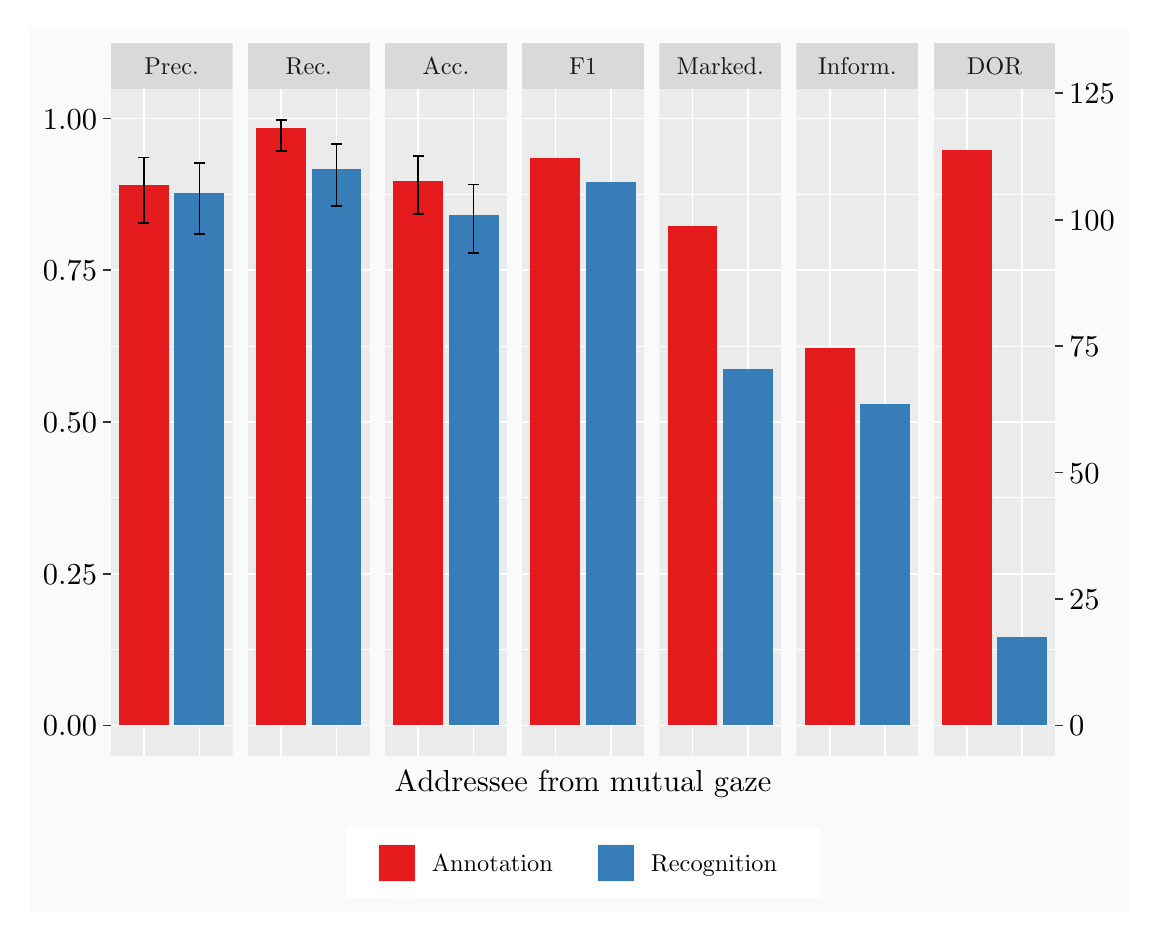
\begin{tikzpicture}[x=1pt,y=1pt]
\definecolor{fillColor}{RGB}{255,255,255}
\path[use as bounding box,fill=fillColor,fill opacity=0.00] (0,0) rectangle (398.34,320.03);
\begin{scope}
\path[clip] (  0.00,  0.00) rectangle (398.34,320.03);
\definecolor{drawColor}{RGB}{255,255,255}
\definecolor{fillColor}{gray}{0.98}

\path[draw=drawColor,line width= 0.6pt,line join=round,line cap=round,fill=fillColor] (  0.00,  0.00) rectangle (398.34,320.03);
\end{scope}
\begin{scope}
\path[clip] ( 30.00, 56.97) rectangle ( 74.06,297.72);
\definecolor{fillColor}{gray}{0.92}

\path[fill=fillColor] ( 30.00, 56.97) rectangle ( 74.06,297.72);
\definecolor{drawColor}{RGB}{255,255,255}

\path[draw=drawColor,line width= 0.3pt,line join=round] ( 30.00, 95.32) --
	( 74.06, 95.32);

\path[draw=drawColor,line width= 0.3pt,line join=round] ( 30.00,150.14) --
	( 74.06,150.14);

\path[draw=drawColor,line width= 0.3pt,line join=round] ( 30.00,204.96) --
	( 74.06,204.96);

\path[draw=drawColor,line width= 0.3pt,line join=round] ( 30.00,259.77) --
	( 74.06,259.77);

\path[draw=drawColor,line width= 0.6pt,line join=round] ( 30.00, 67.92) --
	( 74.06, 67.92);

\path[draw=drawColor,line width= 0.6pt,line join=round] ( 30.00,122.73) --
	( 74.06,122.73);

\path[draw=drawColor,line width= 0.6pt,line join=round] ( 30.00,177.55) --
	( 74.06,177.55);

\path[draw=drawColor,line width= 0.6pt,line join=round] ( 30.00,232.36) --
	( 74.06,232.36);

\path[draw=drawColor,line width= 0.6pt,line join=round] ( 30.00,287.18) --
	( 74.06,287.18);

\path[draw=drawColor,line width= 0.6pt,line join=round] ( 42.02, 56.97) --
	( 42.02,297.72);

\path[draw=drawColor,line width= 0.6pt,line join=round] ( 62.04, 56.97) --
	( 62.04,297.72);
\definecolor{fillColor}{RGB}{228,26,28}

\path[fill=fillColor] ( 33.00, 67.92) rectangle ( 51.03,263.15);
\definecolor{fillColor}{RGB}{55,126,184}

\path[fill=fillColor] ( 53.03, 67.92) rectangle ( 71.05,260.17);
\definecolor{drawColor}{RGB}{0,0,0}

\path[draw=drawColor,line width= 0.6pt,line join=round] ( 60.04,271.08) --
	( 64.04,271.08);

\path[draw=drawColor,line width= 0.6pt,line join=round] ( 62.04,271.08) --
	( 62.04,245.54);

\path[draw=drawColor,line width= 0.6pt,line join=round] ( 60.04,245.54) --
	( 64.04,245.54);

\path[draw=drawColor,line width= 0.6pt,line join=round] ( 40.01,273.16) --
	( 44.02,273.16);

\path[draw=drawColor,line width= 0.6pt,line join=round] ( 42.02,273.16) --
	( 42.02,249.50);

\path[draw=drawColor,line width= 0.6pt,line join=round] ( 40.01,249.50) --
	( 44.02,249.50);
\end{scope}
\begin{scope}
\path[clip] ( 79.56, 56.97) rectangle (123.61,297.72);
\definecolor{fillColor}{gray}{0.92}

\path[fill=fillColor] ( 79.56, 56.97) rectangle (123.61,297.72);
\definecolor{drawColor}{RGB}{255,255,255}

\path[draw=drawColor,line width= 0.3pt,line join=round] ( 79.56, 95.32) --
	(123.61, 95.32);

\path[draw=drawColor,line width= 0.3pt,line join=round] ( 79.56,150.14) --
	(123.61,150.14);

\path[draw=drawColor,line width= 0.3pt,line join=round] ( 79.56,204.96) --
	(123.61,204.96);

\path[draw=drawColor,line width= 0.3pt,line join=round] ( 79.56,259.77) --
	(123.61,259.77);

\path[draw=drawColor,line width= 0.6pt,line join=round] ( 79.56, 67.92) --
	(123.61, 67.92);

\path[draw=drawColor,line width= 0.6pt,line join=round] ( 79.56,122.73) --
	(123.61,122.73);

\path[draw=drawColor,line width= 0.6pt,line join=round] ( 79.56,177.55) --
	(123.61,177.55);

\path[draw=drawColor,line width= 0.6pt,line join=round] ( 79.56,232.36) --
	(123.61,232.36);

\path[draw=drawColor,line width= 0.6pt,line join=round] ( 79.56,287.18) --
	(123.61,287.18);

\path[draw=drawColor,line width= 0.6pt,line join=round] ( 91.57, 56.97) --
	( 91.57,297.72);

\path[draw=drawColor,line width= 0.6pt,line join=round] (111.60, 56.97) --
	(111.60,297.72);
\definecolor{fillColor}{RGB}{228,26,28}

\path[fill=fillColor] ( 82.56, 67.92) rectangle (100.58,283.86);
\definecolor{fillColor}{RGB}{55,126,184}

\path[fill=fillColor] (102.59, 67.92) rectangle (120.61,268.91);
\definecolor{drawColor}{RGB}{0,0,0}

\path[draw=drawColor,line width= 0.6pt,line join=round] (109.59,277.90) --
	(113.60,277.90);

\path[draw=drawColor,line width= 0.6pt,line join=round] (111.60,277.90) --
	(111.60,255.56);

\path[draw=drawColor,line width= 0.6pt,line join=round] (109.59,255.56) --
	(113.60,255.56);

\path[draw=drawColor,line width= 0.6pt,line join=round] ( 89.57,286.78) --
	( 93.57,286.78);

\path[draw=drawColor,line width= 0.6pt,line join=round] ( 91.57,286.78) --
	( 91.57,275.42);

\path[draw=drawColor,line width= 0.6pt,line join=round] ( 89.57,275.42) --
	( 93.57,275.42);
\end{scope}
\begin{scope}
\path[clip] (129.11, 56.97) rectangle (173.17,297.72);
\definecolor{fillColor}{gray}{0.92}

\path[fill=fillColor] (129.11, 56.97) rectangle (173.17,297.72);
\definecolor{drawColor}{RGB}{255,255,255}

\path[draw=drawColor,line width= 0.3pt,line join=round] (129.11, 95.32) --
	(173.17, 95.32);

\path[draw=drawColor,line width= 0.3pt,line join=round] (129.11,150.14) --
	(173.17,150.14);

\path[draw=drawColor,line width= 0.3pt,line join=round] (129.11,204.96) --
	(173.17,204.96);

\path[draw=drawColor,line width= 0.3pt,line join=round] (129.11,259.77) --
	(173.17,259.77);

\path[draw=drawColor,line width= 0.6pt,line join=round] (129.11, 67.92) --
	(173.17, 67.92);

\path[draw=drawColor,line width= 0.6pt,line join=round] (129.11,122.73) --
	(173.17,122.73);

\path[draw=drawColor,line width= 0.6pt,line join=round] (129.11,177.55) --
	(173.17,177.55);

\path[draw=drawColor,line width= 0.6pt,line join=round] (129.11,232.36) --
	(173.17,232.36);

\path[draw=drawColor,line width= 0.6pt,line join=round] (129.11,287.18) --
	(173.17,287.18);

\path[draw=drawColor,line width= 0.6pt,line join=round] (141.13, 56.97) --
	(141.13,297.72);

\path[draw=drawColor,line width= 0.6pt,line join=round] (161.15, 56.97) --
	(161.15,297.72);
\definecolor{fillColor}{RGB}{228,26,28}

\path[fill=fillColor] (132.12, 67.92) rectangle (150.14,264.76);
\definecolor{fillColor}{RGB}{55,126,184}

\path[fill=fillColor] (152.14, 67.92) rectangle (170.16,252.30);
\definecolor{drawColor}{RGB}{0,0,0}

\path[draw=drawColor,line width= 0.6pt,line join=round] (159.15,263.41) --
	(163.16,263.41);

\path[draw=drawColor,line width= 0.6pt,line join=round] (161.15,263.41) --
	(161.15,238.58);

\path[draw=drawColor,line width= 0.6pt,line join=round] (159.15,238.58) --
	(163.16,238.58);

\path[draw=drawColor,line width= 0.6pt,line join=round] (139.13,273.64) --
	(143.13,273.64);

\path[draw=drawColor,line width= 0.6pt,line join=round] (141.13,273.64) --
	(141.13,252.80);

\path[draw=drawColor,line width= 0.6pt,line join=round] (139.13,252.80) --
	(143.13,252.80);
\end{scope}
\begin{scope}
\path[clip] (178.67, 56.97) rectangle (222.72,297.72);
\definecolor{fillColor}{gray}{0.92}

\path[fill=fillColor] (178.67, 56.97) rectangle (222.72,297.72);
\definecolor{drawColor}{RGB}{255,255,255}

\path[draw=drawColor,line width= 0.3pt,line join=round] (178.67, 95.32) --
	(222.72, 95.32);

\path[draw=drawColor,line width= 0.3pt,line join=round] (178.67,150.14) --
	(222.72,150.14);

\path[draw=drawColor,line width= 0.3pt,line join=round] (178.67,204.96) --
	(222.72,204.96);

\path[draw=drawColor,line width= 0.3pt,line join=round] (178.67,259.77) --
	(222.72,259.77);

\path[draw=drawColor,line width= 0.6pt,line join=round] (178.67, 67.92) --
	(222.72, 67.92);

\path[draw=drawColor,line width= 0.6pt,line join=round] (178.67,122.73) --
	(222.72,122.73);

\path[draw=drawColor,line width= 0.6pt,line join=round] (178.67,177.55) --
	(222.72,177.55);

\path[draw=drawColor,line width= 0.6pt,line join=round] (178.67,232.36) --
	(222.72,232.36);

\path[draw=drawColor,line width= 0.6pt,line join=round] (178.67,287.18) --
	(222.72,287.18);

\path[draw=drawColor,line width= 0.6pt,line join=round] (190.68, 56.97) --
	(190.68,297.72);

\path[draw=drawColor,line width= 0.6pt,line join=round] (210.71, 56.97) --
	(210.71,297.72);
\definecolor{fillColor}{RGB}{228,26,28}

\path[fill=fillColor] (181.67, 67.92) rectangle (199.70,272.98);
\definecolor{fillColor}{RGB}{55,126,184}

\path[fill=fillColor] (201.70, 67.92) rectangle (219.72,264.44);
\end{scope}
\begin{scope}
\path[clip] (228.22, 56.97) rectangle (272.28,297.72);
\definecolor{fillColor}{gray}{0.92}

\path[fill=fillColor] (228.22, 56.97) rectangle (272.28,297.72);
\definecolor{drawColor}{RGB}{255,255,255}

\path[draw=drawColor,line width= 0.3pt,line join=round] (228.22, 95.32) --
	(272.28, 95.32);

\path[draw=drawColor,line width= 0.3pt,line join=round] (228.22,150.14) --
	(272.28,150.14);

\path[draw=drawColor,line width= 0.3pt,line join=round] (228.22,204.96) --
	(272.28,204.96);

\path[draw=drawColor,line width= 0.3pt,line join=round] (228.22,259.77) --
	(272.28,259.77);

\path[draw=drawColor,line width= 0.6pt,line join=round] (228.22, 67.92) --
	(272.28, 67.92);

\path[draw=drawColor,line width= 0.6pt,line join=round] (228.22,122.73) --
	(272.28,122.73);

\path[draw=drawColor,line width= 0.6pt,line join=round] (228.22,177.55) --
	(272.28,177.55);

\path[draw=drawColor,line width= 0.6pt,line join=round] (228.22,232.36) --
	(272.28,232.36);

\path[draw=drawColor,line width= 0.6pt,line join=round] (228.22,287.18) --
	(272.28,287.18);

\path[draw=drawColor,line width= 0.6pt,line join=round] (240.24, 56.97) --
	(240.24,297.72);

\path[draw=drawColor,line width= 0.6pt,line join=round] (260.27, 56.97) --
	(260.27,297.72);
\definecolor{fillColor}{RGB}{228,26,28}

\path[fill=fillColor] (231.23, 67.92) rectangle (249.25,248.53);
\definecolor{fillColor}{RGB}{55,126,184}

\path[fill=fillColor] (251.25, 67.92) rectangle (269.28,196.70);
\end{scope}
\begin{scope}
\path[clip] (277.78, 56.97) rectangle (321.84,297.72);
\definecolor{fillColor}{gray}{0.92}

\path[fill=fillColor] (277.78, 56.97) rectangle (321.84,297.72);
\definecolor{drawColor}{RGB}{255,255,255}

\path[draw=drawColor,line width= 0.3pt,line join=round] (277.78, 95.32) --
	(321.84, 95.32);

\path[draw=drawColor,line width= 0.3pt,line join=round] (277.78,150.14) --
	(321.84,150.14);

\path[draw=drawColor,line width= 0.3pt,line join=round] (277.78,204.96) --
	(321.84,204.96);

\path[draw=drawColor,line width= 0.3pt,line join=round] (277.78,259.77) --
	(321.84,259.77);

\path[draw=drawColor,line width= 0.6pt,line join=round] (277.78, 67.92) --
	(321.84, 67.92);

\path[draw=drawColor,line width= 0.6pt,line join=round] (277.78,122.73) --
	(321.84,122.73);

\path[draw=drawColor,line width= 0.6pt,line join=round] (277.78,177.55) --
	(321.84,177.55);

\path[draw=drawColor,line width= 0.6pt,line join=round] (277.78,232.36) --
	(321.84,232.36);

\path[draw=drawColor,line width= 0.6pt,line join=round] (277.78,287.18) --
	(321.84,287.18);

\path[draw=drawColor,line width= 0.6pt,line join=round] (289.80, 56.97) --
	(289.80,297.72);

\path[draw=drawColor,line width= 0.6pt,line join=round] (309.82, 56.97) --
	(309.82,297.72);
\definecolor{fillColor}{RGB}{228,26,28}

\path[fill=fillColor] (280.78, 67.92) rectangle (298.81,204.13);
\definecolor{fillColor}{RGB}{55,126,184}

\path[fill=fillColor] (300.81, 67.92) rectangle (318.83,184.19);
\end{scope}
\begin{scope}
\path[clip] (327.34, 56.97) rectangle (371.39,297.72);
\definecolor{fillColor}{gray}{0.92}

\path[fill=fillColor] (327.34, 56.97) rectangle (371.39,297.72);
\definecolor{drawColor}{RGB}{255,255,255}

\path[draw=drawColor,line width= 0.3pt,line join=round] (327.34, 95.32) --
	(371.39, 95.32);

\path[draw=drawColor,line width= 0.3pt,line join=round] (327.34,150.14) --
	(371.39,150.14);

\path[draw=drawColor,line width= 0.3pt,line join=round] (327.34,204.96) --
	(371.39,204.96);

\path[draw=drawColor,line width= 0.3pt,line join=round] (327.34,259.77) --
	(371.39,259.77);

\path[draw=drawColor,line width= 0.6pt,line join=round] (327.34, 67.92) --
	(371.39, 67.92);

\path[draw=drawColor,line width= 0.6pt,line join=round] (327.34,122.73) --
	(371.39,122.73);

\path[draw=drawColor,line width= 0.6pt,line join=round] (327.34,177.55) --
	(371.39,177.55);

\path[draw=drawColor,line width= 0.6pt,line join=round] (327.34,232.36) --
	(371.39,232.36);

\path[draw=drawColor,line width= 0.6pt,line join=round] (327.34,287.18) --
	(371.39,287.18);

\path[draw=drawColor,line width= 0.6pt,line join=round] (339.35, 56.97) --
	(339.35,297.72);

\path[draw=drawColor,line width= 0.6pt,line join=round] (359.38, 56.97) --
	(359.38,297.72);
\definecolor{fillColor}{RGB}{228,26,28}

\path[fill=fillColor] (330.34, 67.92) rectangle (348.36,275.76);
\definecolor{fillColor}{RGB}{55,126,184}

\path[fill=fillColor] (350.37, 67.92) rectangle (368.39, 99.84);
\end{scope}
\begin{scope}
\path[clip] ( 30.00,297.72) rectangle ( 74.06,314.53);
\definecolor{fillColor}{gray}{0.85}

\path[fill=fillColor] ( 30.00,297.72) rectangle ( 74.06,314.53);
\definecolor{drawColor}{gray}{0.10}

\node[text=drawColor,anchor=base,inner sep=0pt, outer sep=0pt, scale=  0.88] at ( 52.03,303.09) {Prec.};
\end{scope}
\begin{scope}
\path[clip] ( 79.56,297.72) rectangle (123.61,314.53);
\definecolor{fillColor}{gray}{0.85}

\path[fill=fillColor] ( 79.56,297.72) rectangle (123.61,314.53);
\definecolor{drawColor}{gray}{0.10}

\node[text=drawColor,anchor=base,inner sep=0pt, outer sep=0pt, scale=  0.88] at (101.58,303.09) {Rec.};
\end{scope}
\begin{scope}
\path[clip] (129.11,297.72) rectangle (173.17,314.53);
\definecolor{fillColor}{gray}{0.85}

\path[fill=fillColor] (129.11,297.72) rectangle (173.17,314.53);
\definecolor{drawColor}{gray}{0.10}

\node[text=drawColor,anchor=base,inner sep=0pt, outer sep=0pt, scale=  0.88] at (151.14,303.09) {Acc.};
\end{scope}
\begin{scope}
\path[clip] (178.67,297.72) rectangle (222.72,314.53);
\definecolor{fillColor}{gray}{0.85}

\path[fill=fillColor] (178.67,297.72) rectangle (222.72,314.53);
\definecolor{drawColor}{gray}{0.10}

\node[text=drawColor,anchor=base,inner sep=0pt, outer sep=0pt, scale=  0.88] at (200.70,303.09) {F1};
\end{scope}
\begin{scope}
\path[clip] (228.22,297.72) rectangle (272.28,314.53);
\definecolor{fillColor}{gray}{0.85}

\path[fill=fillColor] (228.22,297.72) rectangle (272.28,314.53);
\definecolor{drawColor}{gray}{0.10}

\node[text=drawColor,anchor=base,inner sep=0pt, outer sep=0pt, scale=  0.88] at (250.25,303.09) {Marked.};
\end{scope}
\begin{scope}
\path[clip] (277.78,297.72) rectangle (321.84,314.53);
\definecolor{fillColor}{gray}{0.85}

\path[fill=fillColor] (277.78,297.72) rectangle (321.84,314.53);
\definecolor{drawColor}{gray}{0.10}

\node[text=drawColor,anchor=base,inner sep=0pt, outer sep=0pt, scale=  0.88] at (299.81,303.09) {Inform.};
\end{scope}
\begin{scope}
\path[clip] (327.34,297.72) rectangle (371.39,314.53);
\definecolor{fillColor}{gray}{0.85}

\path[fill=fillColor] (327.34,297.72) rectangle (371.39,314.53);
\definecolor{drawColor}{gray}{0.10}

\node[text=drawColor,anchor=base,inner sep=0pt, outer sep=0pt, scale=  0.88] at (349.36,303.09) {DOR};
\end{scope}
\begin{scope}
\path[clip] (  0.00,  0.00) rectangle (398.34,320.03);
\definecolor{drawColor}{RGB}{0,0,0}

\node[text=drawColor,anchor=base east,inner sep=0pt, outer sep=0pt, scale=  1.10] at ( 25.05, 64.13) {0.00};

\node[text=drawColor,anchor=base east,inner sep=0pt, outer sep=0pt, scale=  1.10] at ( 25.05,118.94) {0.25};

\node[text=drawColor,anchor=base east,inner sep=0pt, outer sep=0pt, scale=  1.10] at ( 25.05,173.76) {0.50};

\node[text=drawColor,anchor=base east,inner sep=0pt, outer sep=0pt, scale=  1.10] at ( 25.05,228.58) {0.75};

\node[text=drawColor,anchor=base east,inner sep=0pt, outer sep=0pt, scale=  1.10] at ( 25.05,283.39) {1.00};
\end{scope}
\begin{scope}
\path[clip] (  0.00,  0.00) rectangle (398.34,320.03);
\definecolor{drawColor}{gray}{0.20}

\path[draw=drawColor,line width= 0.6pt,line join=round] ( 27.25, 67.92) --
	( 30.00, 67.92);

\path[draw=drawColor,line width= 0.6pt,line join=round] ( 27.25,122.73) --
	( 30.00,122.73);

\path[draw=drawColor,line width= 0.6pt,line join=round] ( 27.25,177.55) --
	( 30.00,177.55);

\path[draw=drawColor,line width= 0.6pt,line join=round] ( 27.25,232.36) --
	( 30.00,232.36);

\path[draw=drawColor,line width= 0.6pt,line join=round] ( 27.25,287.18) --
	( 30.00,287.18);
\end{scope}
\begin{scope}
\path[clip] (  0.00,  0.00) rectangle (398.34,320.03);
\definecolor{drawColor}{gray}{0.20}

\path[draw=drawColor,line width= 0.6pt,line join=round] (371.39, 67.92) --
	(374.14, 67.92);

\path[draw=drawColor,line width= 0.6pt,line join=round] (371.39,113.60) --
	(374.14,113.60);

\path[draw=drawColor,line width= 0.6pt,line join=round] (371.39,159.28) --
	(374.14,159.28);

\path[draw=drawColor,line width= 0.6pt,line join=round] (371.39,204.96) --
	(374.14,204.96);

\path[draw=drawColor,line width= 0.6pt,line join=round] (371.39,250.64) --
	(374.14,250.64);

\path[draw=drawColor,line width= 0.6pt,line join=round] (371.39,296.32) --
	(374.14,296.32);
\end{scope}
\begin{scope}
\path[clip] (  0.00,  0.00) rectangle (398.34,320.03);
\definecolor{drawColor}{RGB}{0,0,0}

\node[text=drawColor,anchor=base west,inner sep=0pt, outer sep=0pt, scale=  1.10] at (376.34, 64.13) {0};

\node[text=drawColor,anchor=base west,inner sep=0pt, outer sep=0pt, scale=  1.10] at (376.34,109.81) {25};

\node[text=drawColor,anchor=base west,inner sep=0pt, outer sep=0pt, scale=  1.10] at (376.34,155.49) {50};

\node[text=drawColor,anchor=base west,inner sep=0pt, outer sep=0pt, scale=  1.10] at (376.34,201.17) {75};

\node[text=drawColor,anchor=base west,inner sep=0pt, outer sep=0pt, scale=  1.10] at (376.34,246.85) {100};

\node[text=drawColor,anchor=base west,inner sep=0pt, outer sep=0pt, scale=  1.10] at (376.34,292.53) {125};
\end{scope}
\begin{scope}
\path[clip] (  0.00,  0.00) rectangle (398.34,320.03);
\definecolor{drawColor}{RGB}{0,0,0}

\node[text=drawColor,anchor=base,inner sep=0pt, outer sep=0pt, scale=  1.10] at (200.70, 43.90) {Addressee from mutual gaze};
\end{scope}
\begin{scope}
\path[clip] (  0.00,  0.00) rectangle (398.34,320.03);
\definecolor{fillColor}{RGB}{255,255,255}

\path[fill=fillColor] (115.08,  5.50) rectangle (286.31, 30.95);
\end{scope}
\begin{scope}
\path[clip] (  0.00,  0.00) rectangle (398.34,320.03);
\definecolor{drawColor}{RGB}{255,255,255}
\definecolor{fillColor}{gray}{0.95}

\path[draw=drawColor,line width= 0.6pt,line join=round,line cap=round,fill=fillColor] (126.08, 11.00) rectangle (140.54, 25.45);
\end{scope}
\begin{scope}
\path[clip] (  0.00,  0.00) rectangle (398.34,320.03);
\definecolor{fillColor}{RGB}{228,26,28}

\path[fill=fillColor] (126.79, 11.71) rectangle (139.82, 24.74);
\end{scope}
\begin{scope}
\path[clip] (  0.00,  0.00) rectangle (398.34,320.03);
\definecolor{drawColor}{RGB}{255,255,255}
\definecolor{fillColor}{gray}{0.95}

\path[draw=drawColor,line width= 0.6pt,line join=round,line cap=round,fill=fillColor] (205.28, 11.00) rectangle (219.73, 25.45);
\end{scope}
\begin{scope}
\path[clip] (  0.00,  0.00) rectangle (398.34,320.03);
\definecolor{fillColor}{RGB}{55,126,184}

\path[fill=fillColor] (205.99, 11.71) rectangle (219.02, 24.74);
\end{scope}
\begin{scope}
\path[clip] (  0.00,  0.00) rectangle (398.34,320.03);
\definecolor{drawColor}{RGB}{0,0,0}

\node[text=drawColor,anchor=base west,inner sep=0pt, outer sep=0pt, scale=  0.88] at (146.04, 15.20) {Annotation};
\end{scope}
\begin{scope}
\path[clip] (  0.00,  0.00) rectangle (398.34,320.03);
\definecolor{drawColor}{RGB}{0,0,0}

\node[text=drawColor,anchor=base west,inner sep=0pt, outer sep=0pt, scale=  0.88] at (225.23, 15.20) {Recognition};
\end{scope}
\end{tikzpicture}
